\section{Versuchsaufbau}
\label{sec:Versuchaufbau}
Für die Messung wird ein Alibava EASy Detekorsystem verwendet. Es
besteht aus einer Detektoreinheit, einer
Kontrolleinheit und einem Computer.
\subsection{Die Detekoreinheit}
Als Detektoreinheit wird ein Halbleitersensor mit
entsprechnender Ausleseelektronik verwendet.
Der Siliziumsensor ist in 128 Streifen unterteilt, jeder ist über
ein Wirebond mit dem Auslesechip (BEETLE) verbunden. Der
BEETLE Chip dient zur Verstärkung des eingehenden Ladungssignals und Umwandlung in eine Auslesespannung.\\
\subsection{Der Halbleitersensor}
Eine schematische Darstellung des verwendeten Sensors ist in Abbildung
\ref{sensor} dargestellt.
\begin{figure}[H]
  \centering
  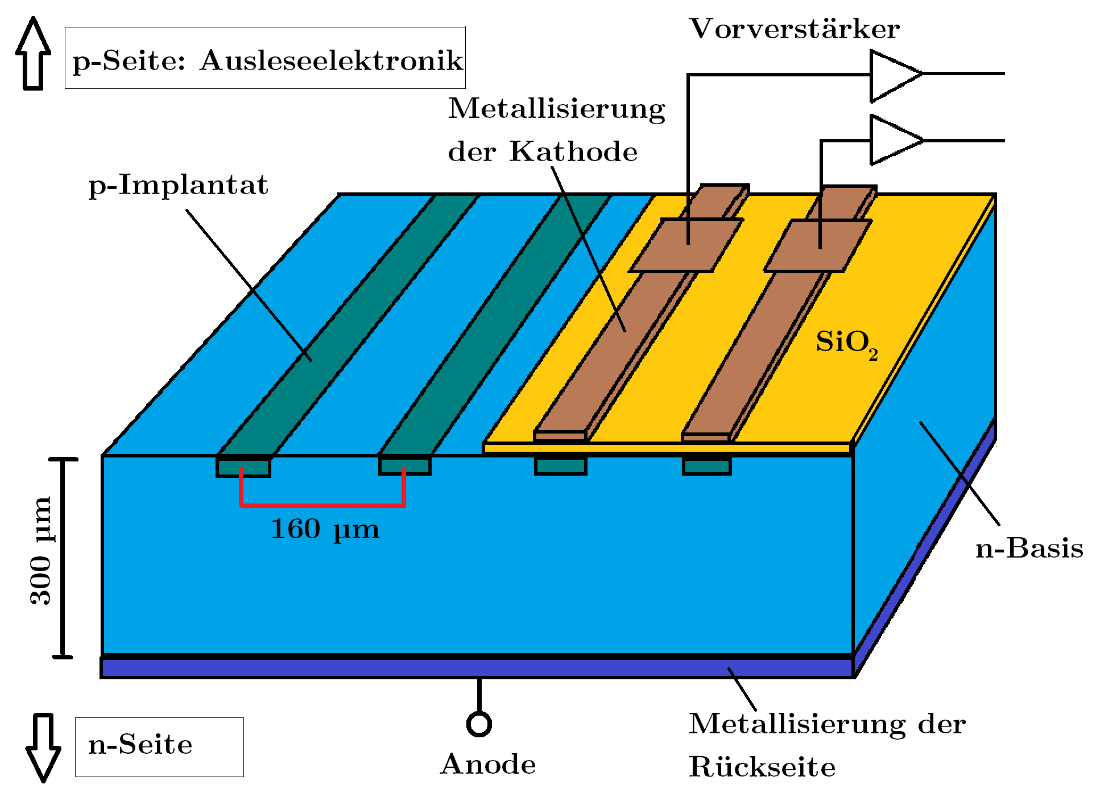
\includegraphics[width=0.81\textwidth]{ressources/sensor.png}
  \caption{Schematische Darstellung des p-in-n-Sensors. \cite{skript}}
  \label{sensor}
\end{figure}
Der pn-Übergang wird hier durch eine n-dotierte Bodenplatte
mit einzelnen p-Implantaten realisiert. In dieser Kombination wird der Sensor als p-in-n Sensor bezeichnet. Durch die stark unterschiedlich dotierten Schichten entsteht ein stark asymmetrisches Verhältnis zwischen den Akzeptoren und Donatoren. \\
Die n-dotierte Siliziumschicht hat eine Dicke von $300\,\mu m$, die p-Implantate sind von einander isoliert um eine
genaue Ortsauflösung zu ermöglichen. Des Weiteren sind die Implantate
kapazitiv mit einer Elektrode aus Aluminium gekoppelt, was über ein ohmschen Kontakt
ausgelesen werden kann.


Der Sensor muss für die Messung voll depletiert sein, da sonst Elektron-Loch-Paare
außerhalb der Depletionszone rekombinieren. Dies hätte zur Folge, dass nicht jedes einfallende Teilchen durch den Sensor detektiert wird. Die Effizienz der Ladungssammlung
$CCE$ steigt mit der Dicke $D$ der Depletionszone, bis die Depletionsspannung erreicht ist.
Im Versuch soll die $CCE$ mit Hilfe eines Lasers und einer $\beta$-Quelle untersucht werden. Hierfür ist die
Eindringtiefe des Laser in Silizium $a$ relevant. Der Zusammenhang ist gegeben durch:

\begin{equation}
    \label{CCE}
    CCE(U)=\frac{1-\exp(\frac{-d_c(U)}{a})}{1-\exp(\frac{-D}{a})}
\end{equation}
Die Eindringtiefe eines Laser der Wellenlänge von 960$\,$nm \cite{skript} hat eine Eindringtiefe
von $d \approx 74\,\mu$m, wobei dieser Wert vom  Material und der Wellenlänge abhängt.
